\documentclass[11pt]{article}

\usepackage[margin=1in]{geometry}
\usepackage{graphicx}
\usepackage{xcolor}
\usepackage{listings}
\usepackage{booktabs}
\usepackage{enumitem}
\usepackage{amsmath}
\usepackage{amssymb}
\usepackage{microtype}                 % better justification -> fewer overfull lines
\setlength{\emergencystretch}{3em}     % last-resort stretch so long code tokens don't overflow
\usepackage[colorlinks=true,linkcolor=blue,urlcolor=blue]{hyperref}

% ---- colors + code styles ---------------------------------------------------
\definecolor{codebg}{RGB}{245,246,248}
\definecolor{codekw}{RGB}{0,90,160}
\definecolor{codestr}{RGB}{160,60,20}
\definecolor{codecom}{RGB}{110,120,130}

\lstdefinestyle{py}{
  language=Python, backgroundcolor=\color{codebg}, basicstyle=\ttfamily\small,
  keywordstyle=\color{codekw}\bfseries, stringstyle=\color{codestr},
  commentstyle=\color{codecom}\itshape, showstringspaces=false, breaklines=true,
  frame=single, rulecolor=\color{gray!40}, columns=fullflexible, tabsize=4,
}
\lstdefinestyle{plain}{
  backgroundcolor=\color{codebg}, basicstyle=\ttfamily\small, showstringspaces=false,
  breaklines=true, frame=single, rulecolor=\color{gray!40}, columns=fullflexible,
}
\lstset{style=py}
\newcommand{\code}[1]{\lstinline[style=plain]|#1|}

\title{\textbf{Online NMR Fitter}\\[2pt]\large Operator's Guide \& Data-Stream Reference}
\author{UNH Polarized Target Group}
\date{\today}

\begin{document}
\maketitle
\tableofcontents
\bigskip

% =============================================================================
\section{What this program is}

The \textbf{Online NMR Fitter} (\code{online_fitter}) fits deuteron (spin-1) NMR sweeps
\emph{live} during a cool-down. LabVIEW's VME loop streams each baseline-subtracted sweep to
the fitter over a local (loopback) network connection; the fitter runs the Dulya spin-1
lineshape fit --- M.\ McClellan's updated version, which includes the phase --- and shows the
polarizations $P$ and $Q$ in real time. It also
\textbf{broadcasts} every fitted result so other programs can use the numbers (see
Section~\ref{sec:stream}).

Nothing here touches the lab LAN: all connections are on \code{127.0.0.1} (``this computer''
only), so the VME crate and the RF switches are never affected.

% =============================================================================
\section{Starting and stopping the fitter}

The fitter is normally launched automatically by the cool-down VI, but you can also run it by
hand from a command prompt in the folder that contains \code{online_fitter}:

\begin{lstlisting}[style=plain]
python -m online_fitter.run
\end{lstlisting}

That single command opens the GUI, starts the loopback server LabVIEW connects to
(\code{127.0.0.1:8777}), and starts the broadcast stream (\code{127.0.0.1:8778}). Useful options:

\begin{itemize}[nosep]
  \item \code{--replace} --- before starting, stop any fitter already running (used by the
        LabVIEW ``Restart Fitter'' button). Leaves every other Python program alone.
  \item \code{--no-publish} --- turn the broadcast stream off (it is on by default).
  \item \code{--material ND3} --- start on a given material.
  \item \code{--dpi-mode system} --- change multi-monitor scaling (default \code{unaware}).
\end{itemize}

To stop it, close the window (or, from LabVIEW, use Restart Fitter). If a fitter ever gets
stuck, \code{python -m online_fitter.stop} force-stops only the fitter.

% =============================================================================
\section{The window at a glance}
\label{sec:window}

\begin{figure}[h!]
  \centering
  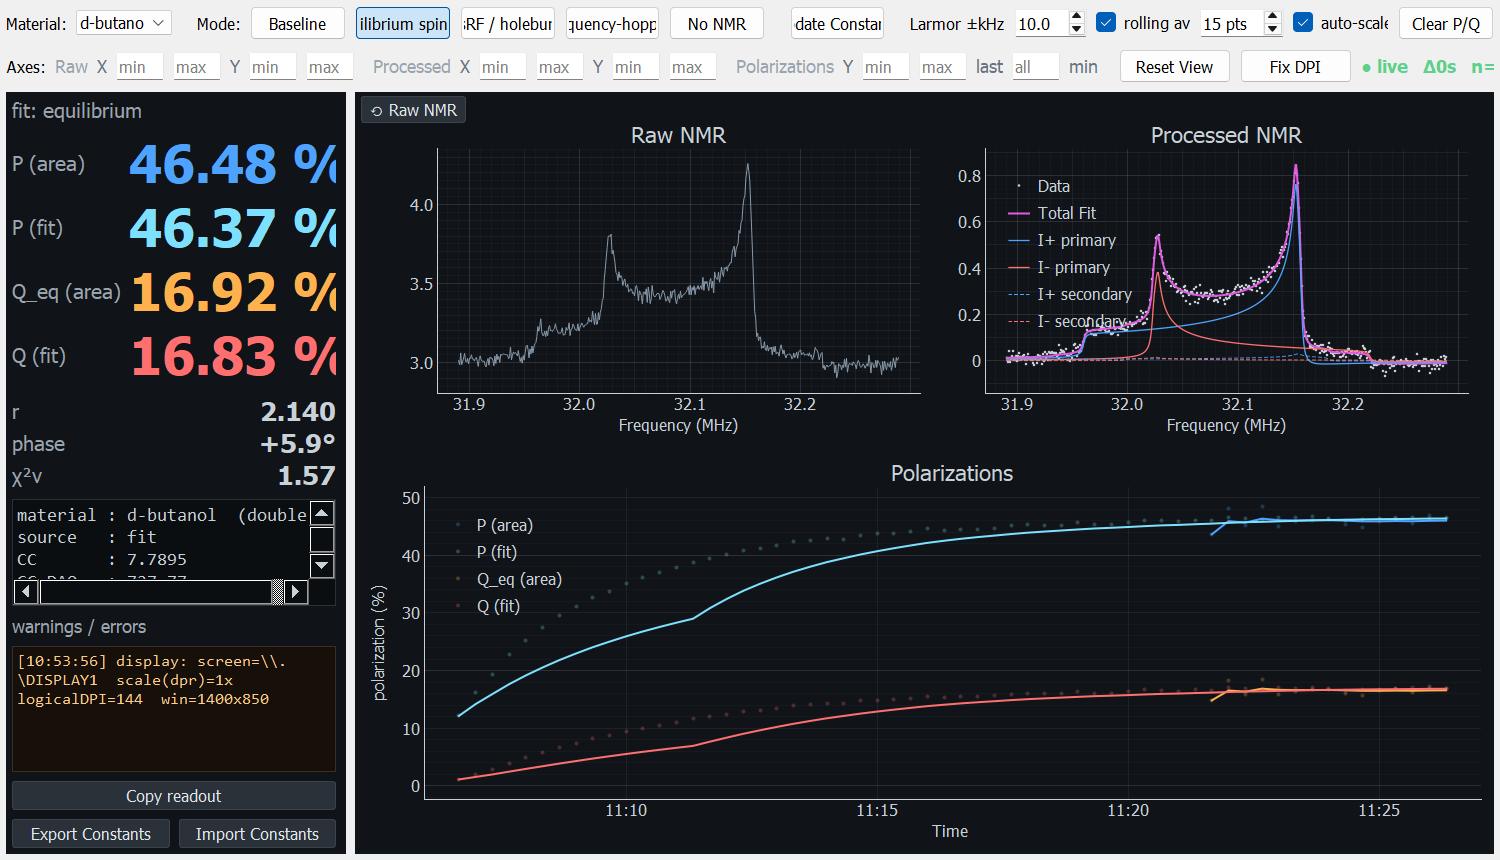
\includegraphics[width=\textwidth]{figures/fig_overview.png}
  \caption{The fitter in \emph{Equilibrium spin-up} mode after \emph{Update Constants}. Left
    readout panel: the large $P$/$Q$ values, the live fit parameters, and the calibration
    constants. Top plots: the raw sweep (left) and the processed data with the total fit and
    the per-nucleus components (right). Bottom: the $P$/$Q$ vs.\ time strip chart. (Figures use
    representative example data.)}
  \label{fig:overview}
\end{figure}

Referring to Figure~\ref{fig:overview}, the window has four regions:

\paragraph{Top control row.} \textbf{Material} selector; the five \textbf{mode} buttons
(Baseline $\,\cdot\,$ Equilibrium spin-up $\,\cdot\,$ ssRF/holeburn $\,\cdot\,$
Frequency-hopping $\,\cdot\,$ No NMR); \textbf{Update Constants}; the \textbf{Larmor $\pm$kHz}
box (for ssRF); the rolling-average and auto-scale toggles; and \textbf{Clear P/Q}.

\paragraph{Second control row.} Manual \textbf{axis limits} for each plot (type a number,
press Enter), \textbf{Reset View} (back to auto-range), \textbf{Fix DPI} (re-render at the
current monitor's scale), and the \textbf{live indicator} on the far right: green
\textcolor{green!60!black}{$\bullet$ live} with the seconds since the last sweep and the sweep
count \code{n}, or red \textbf{$\bullet$ NO DATA} if sweeps stop arriving.

\paragraph{Left readout panel.} The big $P$ and $Q$ values (area method and fit method), the
live per-sweep fit parameters ($r$, phase, $\chi^2_\nu$), the calibration constants (including
\code{CC} and \code{CC_DAQ}), a warnings box, and the \textbf{Copy readout} /
\textbf{Export Constants} / \textbf{Import Constants} buttons.

\paragraph{Plots.} Two spectra on top --- \textbf{Raw NMR} (as digitized) and
\textbf{Processed NMR} (baseline-subtracted data + total fit + I+/I$-$ components) --- and the
\textbf{Polarizations} strip chart along the bottom. The small button in the top-left corner of
the left plot cycles what that plot shows (Section~\ref{sec:leftview}).

% =============================================================================
\section{Operating procedure}

\begin{enumerate}[nosep]
  \item \textbf{Pick the material} (d-butanol, d-propanediol, or ND3) from the selector. This
        loads that material's preset lineshape constants as a starting point.
  \item \textbf{Choose the mode} for what the target is doing:
    \begin{itemize}[nosep]
      \item \textbf{Equilibrium spin-up} --- the normal polarizing mode; fits each sweep for $P$.
      \item \textbf{ssRF / holeburn} --- hole-burnt lineshape; reads $r_{\text{eq}}$ from the
            Larmor region (set the half-width in \textbf{Larmor $\pm$kHz}; 0 uses the reference).
      \item \textbf{Frequency-hopping} --- independent $r_N$, $r_P$.
      \item \textbf{Baseline} / \textbf{No NMR} --- display-only; no polarization is reported.
    \end{itemize}
  \item \textbf{Let signal build}, then click \textbf{Update Constants} (next section).
  \item \textbf{Read $P$ and $Q$} from the left panel and watch the strip chart.
\end{enumerate}

% -----------------------------------------------------------------------------
\subsection{Update Constants (calibration)}

\textbf{Update Constants} runs the full open fit over the average of the last $\sim$10
equilibrium sweeps, refreshes every lineshape constant, and sets the area calibration
constants \code{CC} and \code{CC_DAQ}. Do it once you have a clean, high-polarization
equilibrium plateau (let the buffer fill with good sweeps first). The fit takes tens of
seconds and \emph{does not} interrupt streaming --- data keeps flowing throughout, and the new
constants swap in atomically at the end. Click the button again (it reads \textbf{Stop} while
running) to abort without changing anything.

To \textbf{check that the fit succeeded}, click the corner button on the left plot until it
reads \textbf{Averaged + Fit for Constants} (Figure~\ref{fig:avgfit}). This shows the exact
averaged data the fit used, with the total fit and the I+/I$-$ components overlaid. A good fit
hugs the data; a bad one is obvious at a glance.

\begin{figure}[h!]
  \centering
  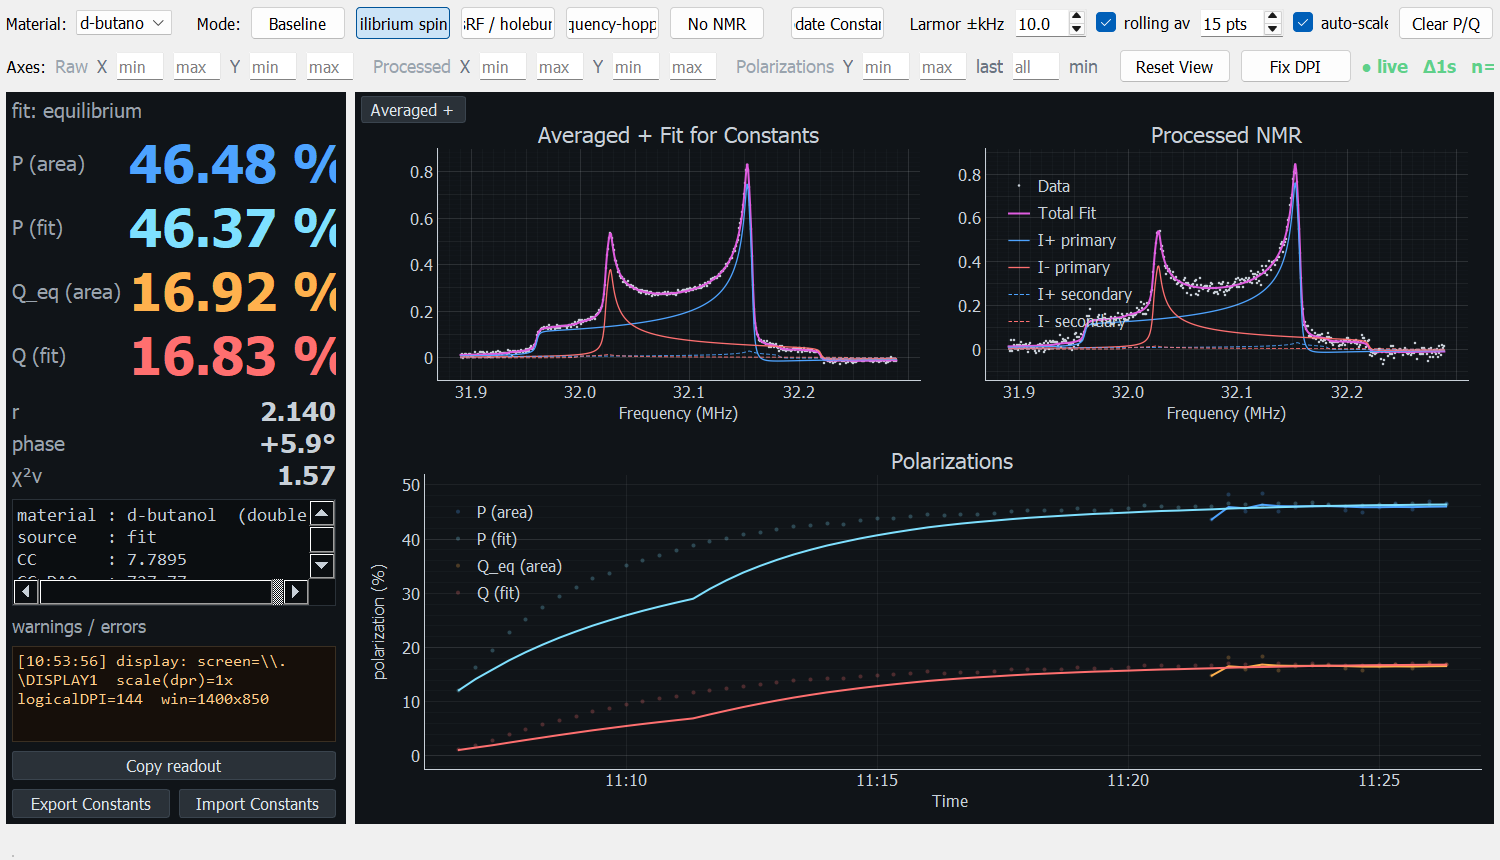
\includegraphics[width=\textwidth]{figures/fig_avgfit.png}
  \caption{The left plot toggled to \textbf{Averaged + Fit for Constants}: the averaged
    equilibrium data (dots) that Update Constants fit, with the total fit (magenta) and the
    per-nucleus components. Use it to judge fit quality after calibrating.}
  \label{fig:avgfit}
\end{figure}

% -----------------------------------------------------------------------------
\subsection{Reading the values: P, Q, and the two CCs}
\label{sec:readout}

\begin{figure}[h!]
  \centering
  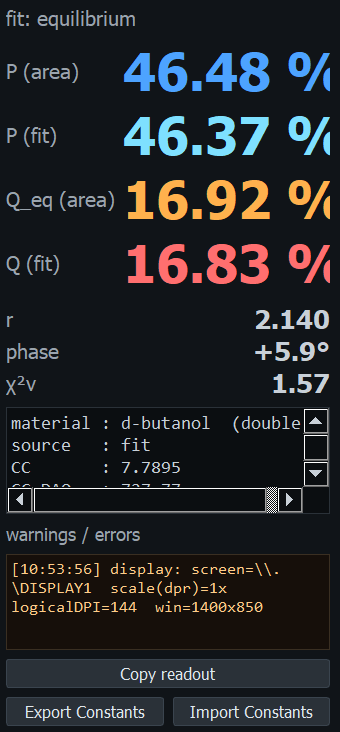
\includegraphics[width=0.42\textwidth]{figures/fig_readout.png}
  \caption{The readout panel. Large values: $P$/$Q$ by area and by fit. Below: the live fit
    parameters and the calibration constants, including \code{CC} and \code{CC_DAQ}.}
  \label{fig:readout}
\end{figure}

The panel (Figure~\ref{fig:readout}) shows two independent measures of polarization:
\begin{itemize}[nosep]
  \item \textbf{P (fit) / Q (fit)} --- from the lineshape fit of each sweep.
  \item \textbf{P (area) / Q\_eq (area)} --- from the calibrated area of the line
        ($P_{\text{area}} = \mathrm{CC}\times\mathrm{area}$), available only after Update Constants.
\end{itemize}
All are in \textbf{percent}. Below them are the live per-sweep $r$, phase, and $\chi^2_\nu$, and
the constants block.

\paragraph{\code{CC} vs.\ \code{CC_DAQ}.} Both are area calibrations, but computed two ways:
\begin{itemize}[nosep]
  \item \code{CC} --- the fitter's own calibration: a trapezoidal integral of the
        \emph{cubic-wing-flattened} line. Gives $P$ as a fraction internally.
  \item \code{CC_DAQ} --- matches the \textbf{LabVIEW DAQ}'s area method: a plain rectangular
        sum of the baseline-subtracted $y$-values times the frequency-bin width, scaled so that
        \code{CC_DAQ} $\times$ (area) $= P$ in \emph{percent}. This is the number to paste into
        the DAQ's own CC field so the DAQ's $P$ matches the fitter.
\end{itemize}
They differ (typically by $\sim$50$\times$) because they use different area definitions and
units; that is expected.

\textbf{Copy readout} copies everything (values + constants) to the clipboard.

% -----------------------------------------------------------------------------
\subsection{The left-plot view toggle}
\label{sec:leftview}

The small button in the top-left corner of the left plot cycles it through:
\begin{enumerate}[nosep]
  \item \textbf{Raw NMR} --- the raw sweep, live.
  \item \textbf{Baseline-subtracted} --- the baseline-subtracted line LabVIEW sends, live.
  \item \textbf{Averaged + Fit for Constants} --- the averaged data + fit from the last
        Update Constants (static; refreshes when you re-calibrate). Use it to judge the fit.
\end{enumerate}

% -----------------------------------------------------------------------------
\subsection{Saving and reusing a calibration}

\textbf{Export Constants} writes the current calibration (all lineshape constants, \code{CC},
\code{CC_DAQ}) plus a reference record (the data date/time and the $P$/$Q$/$r$/phase/$\chi^2_\nu$
at the time) to a file under \code{online_fitter/constants/}. \textbf{Import Constants} loads
such a file and installs it \emph{exactly as if you had just run Update Constants} (the
reference values are ignored on load). Useful to restore a known-good calibration at the start
of a run.

% -----------------------------------------------------------------------------
\subsection{View controls, restart, and troubleshooting}

\begin{itemize}[nosep]
  \item \textbf{Axis limits}: type numbers into the second-row boxes to fix a plot's range;
        \textbf{Reset View} returns all plots to auto-range. (Mouse wheel-zoom is disabled.)
  \item \textbf{Fix DPI}: if plots look clipped after dragging the window to another monitor,
        click this. It also prints the monitor/scale into the warnings box.
  \item \textbf{Restart Fitter} (LabVIEW, lower-right of the cool-down VI front panel;
        Figure~\ref{fig:restart}): stops the old fitter and starts a fresh one; the VI
        reconnects on its own.
  \item \textbf{Live indicator}: red \textbf{NO DATA} means sweeps stopped arriving. The
        fitter also writes \code{online_fitter/logs/online_fitter.log} --- connection events and
        a 60-second heartbeat --- which is the first place to look if a run stalls.
\end{itemize}

\begin{figure}[h!]
  \centering
  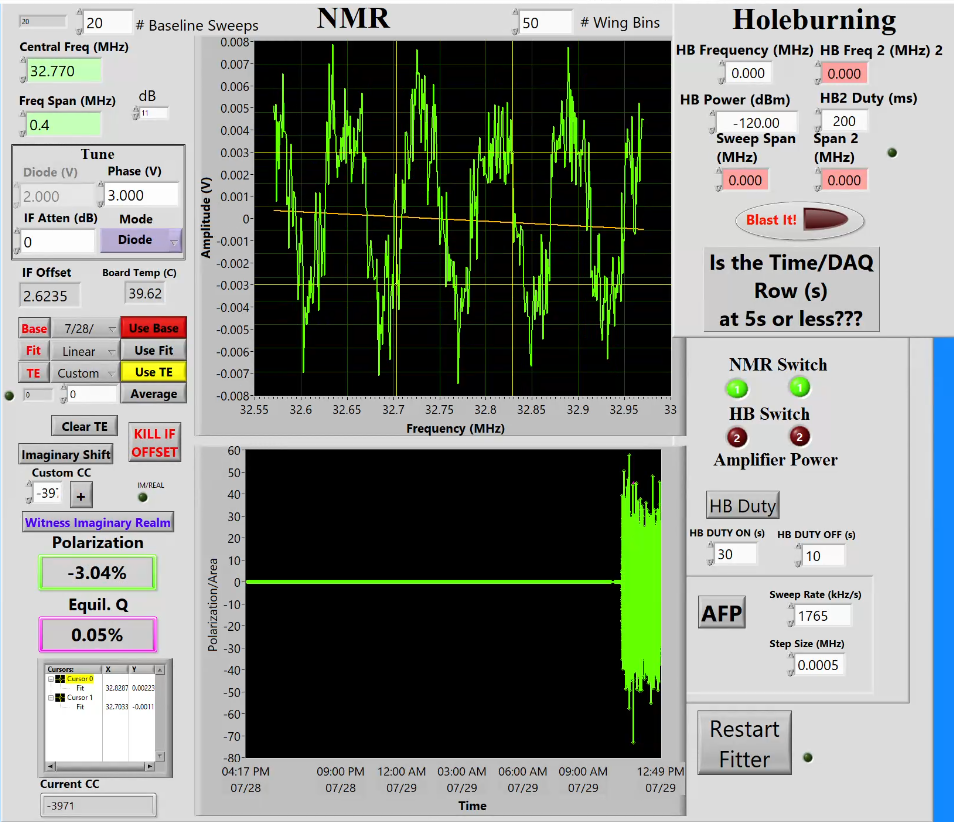
\includegraphics[width=0.75\textwidth]{figures/fig_labview_restart.png}
  \caption{The cool-down VI's LabVIEW front panel. The \textbf{Restart Fitter} button is at the
    lower-right; use it to cleanly stop and relaunch the fitter (the VI reconnects on its own).}
  \label{fig:restart}
\end{figure}

% =============================================================================
\section{Reading the exported data stream}
\label{sec:stream}

This section assumes \emph{no background}: it explains, from scratch, how another program reads
the fitter's live results. A complete, runnable example ships with the code as
\code{online_fitter/example_data_reader.py}.

% -----------------------------------------------------------------------------
\subsection{The idea in three steps}

\begin{enumerate}[nosep]
  \item \textbf{A socket is a pipe between two programs.} While it runs, the fitter keeps one
        end of a pipe open on \emph{this computer} at address \code{127.0.0.1} (``localhost''),
        port \code{8778}. Your program is the \emph{client}: it connects to that address and
        then just reads.
  \item \textbf{The fitter sends NDJSON} = ``newline-delimited JSON'': one JSON object per line,
        each line ending in a newline. So you read the pipe one line at a time, and each line is
        one fitted sweep.
  \item \textbf{Each line is a JSON object.} In Python, \code{json.loads(line)} turns that line
        of text into an ordinary dictionary; then you read values by name, e.g.
        \code{msg["P_fit"]}.
\end{enumerate}

You do \emph{not} need the fitter's source to consume the stream --- only Python's standard
library (\code{socket} and \code{json}).

% -----------------------------------------------------------------------------
\subsection{What each line contains}

Every line carries four groups of data, in this order:

\begin{enumerate}[nosep]
  \item \textbf{Good fit constants} --- \code{msg["constants"]} (the calibration: \code{CC},
        \code{CC_DAQ}, and the lineshape constants). The flag \code{msg["constants_good"]} is
        \code{true} only after the operator has run Update Constants (or imported constants);
        until then the constants are preset seeds. \emph{It is good practice to wait for
        \code{constants_good == true} before trusting the numbers.}
  \item \textbf{Processed NMR data} --- \code{msg["data"]} (the cubic-subtracted line).
  \item \textbf{Processed NMR fit} --- \code{msg["total_fit"]} and the four components
        \code{I_plus_primary}, \code{I_minus_primary}, \code{I_plus_secondary},
        \code{I_minus_secondary}. For single-bond \textbf{ND3} the two secondaries are all zeros.
  \item \textbf{Raw NMR} --- \code{msg["raw"]} (the sweep as LabVIEW sent it).
\end{enumerate}

Every array above lines up sample-for-sample with the frequency axis
\code{msg["freqs_mhz"]} (same length, same order). Also on each line: this sweep's
polarizations (\code{P_area}, \code{P_fit}, \code{Q_eq}, \code{Q_fit}, \code{r},
\code{phase_deg}, \code{red_chisq}) and \code{material}, \code{model}, \code{fit_type},
\code{npts}, \code{ts}.

\paragraph{About \code{null}.} JSON has no ``NaN''. Any sample the fitter could not compute
(for example, component curves while in Baseline/No-NMR mode) is sent as JSON \code{null},
which becomes Python \code{None}. Turn it into \code{float('nan')} when building arrays.

One line looks like this (arrays abbreviated):
\begin{lstlisting}[style=plain]
{"type":"fit","ts":"6/17/2026 9:31:27 PM","fit_type":"equilibrium","mode":"equilibrium",
 "material":"d-butanol","model":"double","npts":451,
 "freqs_mhz":[...], "P_fit":46.4,"Q_fit":16.8,"r":2.14,"phase_deg":5.9,"red_chisq":1.6,
 "constants_good":true,
 "constants":{"source":"fit","CC":7.79,"CC_DAQ":727.8,"omegD":32.09, ... ,"r":2.14},
 "data":[...], "total_fit":[...],
 "I_plus_primary":[...],"I_minus_primary":[...],
 "I_plus_secondary":[...],"I_minus_secondary":[...],
 "raw":[...]}
\end{lstlisting}

% -----------------------------------------------------------------------------
\subsection{The minimal reader}

The core of a consumer is only a few lines: open the pipe, read it line by line, and turn each
line into a dictionary. This is the heart of \code{example_data_reader.py}:

\begin{lstlisting}
import socket, json

with socket.create_connection(("127.0.0.1", 8778), timeout=30) as sock:
    stream = sock.makefile("rb")        # read the pipe like a file, one line at a time
    for raw_line in stream:             # each iteration = the next sweep
        raw_line = raw_line.strip()
        if not raw_line:
            continue
        msg = json.loads(raw_line)      # text line -> Python dict
        # --- your logic here ---
        if msg["constants_good"]:
            print("CC_DAQ =", msg["constants"]["CC_DAQ"], " P_fit =", msg["P_fit"])
\end{lstlisting}

To turn a number list (which may contain \code{None}) into a clean numpy array:

\begin{lstlisting}
import numpy as np

def to_array(values):
    if values is None:
        return None
    return np.asarray([float("nan") if v is None else float(v) for v in values], float)

freqs = to_array(msg["freqs_mhz"])
data  = to_array(msg["data"])          # both share the same length and order
\end{lstlisting}

% -----------------------------------------------------------------------------
\subsection{Running the example}

\begin{lstlisting}[style=plain]
# 1. start the fitter (it broadcasts by default):
python -m online_fitter.run
# 2. in a second terminal, run the example reader:
python -m online_fitter.example_data_reader
\end{lstlisting}

The example prints one summary line per fitted sweep, showing all four groups. Copy that file
and replace the body of \code{handle_message(...)} with your own logic --- write to a file,
push to EPICS, plot, whatever your application needs. Its comments walk through every field.

% -----------------------------------------------------------------------------
\subsection{Field reference}

\begin{table}[h!]
  \centering
  \small
  \begin{tabular}{@{}lll@{}}
    \toprule
    \textbf{Field} & \textbf{Type} & \textbf{Meaning} \\
    \midrule
    \code{ts}                 & string      & LabVIEW timestamp of the sweep \\
    \code{material}, \code{model} & string  & e.g.\ \code{d-butanol}, \code{double} (or \code{single} = ND3) \\
    \code{fit_type}, \code{mode}  & string  & the fit routine used / the operator's mode \\
    \code{npts}               & int         & length of every array below \\
    \code{freqs_mhz}          & list        & frequency axis (MHz); shared by all arrays \\
    \code{P_area}, \code{P_fit}   & number  & polarization (\%), area \& fit methods \\
    \code{Q_eq}, \code{Q_fit}     & number  & tensor polarization (\%) \\
    \code{r}, \code{phase_deg}, \code{red_chisq} & number & this sweep's fit params \\
    \code{constants_good}     & bool        & \code{true} once calibrated (Update Constants/import) \\
    \code{constants}          & object      & \code{CC}, \code{CC_DAQ}, \code{source}, lineshape constants \\
    \code{data}               & list        & processed (cubic-subtracted) NMR line \\
    \code{total_fit}          & list        & total fitted lineshape \\
    \code{I_plus_primary}, \code{I_minus_primary}   & list & primary-bond components \\
    \code{I_plus_secondary}, \code{I_minus_secondary} & list & secondary components (0 for ND3) \\
    \code{raw}                & list        & raw NMR sweep \\
    \bottomrule
  \end{tabular}
  \caption{Fields on each broadcast line. Any non-finite sample inside a list is JSON \code{null}.}
\end{table}

\paragraph{Notes.}
\begin{itemize}[nosep]
  \item \textbf{Same computer only.} The stream is loopback (\code{127.0.0.1}); a consumer on
        another machine cannot reach it without a relay.
  \item \textbf{Many readers at once} are fine --- connect as many as you like.
  \item \textbf{Never blocks the fitter.} A slow or disconnected reader is simply dropped; it
        can never stall the fit or the acquisition.
\end{itemize}

\end{document}
